%----------------------------------------------------------------------------------------
%    PACKAGES AND THEMES
%----------------------------------------------------------------------------------------

\documentclass[aspectratio=169,xcolor=dvipsnames]{beamer}
\usetheme{SimplePlus}
\usepackage{hyperref}
\usepackage{graphicx} % Allows including images
\usepackage{booktabs} % Allows the use of \toprule, \midrule and \bottomrule in tables

\usepackage{tikz}

\usepackage{amsmath} % For math equations
\usepackage{verbatim}
\usetikzlibrary{arrows,shapes}
\usetikzlibrary{arrows.meta, positioning} % Required TikZ libraries for the diagram

\setbeamerfont{alerted text}{series=\bfseries} % Make alert text bold
\setbeamercolor{alerted text}{fg=black} % Set alert text color to black (optional, to remove red)

\setbeamertemplate{footline}{
    \hbox{%
        \begin{beamercolorbox}[wd=\paperwidth, ht=2.5ex, dp=1ex, left]{footline}%
            \hspace{1em}Technion - Israel Institute of Technology
            \hfill Design Management Noncooperative Communication Networks
            \hfill \ Jan 2025
            \hfill \insertframenumber{} / \inserttotalframenumber%
            \hspace{1em}
        \end{beamercolorbox}%
    }
}

\date{} % Explicitly suppress the date

%----------------------------------------------------------------------------------------
%    TITLE PAGE
%----------------------------------------------------------------------------------------

\title{AoI-Guaranteed Incentive Mechanism for Mobile
Crowdsensing With Freshness Concerns}
% \subtitle{Subtitle}

\author{Yin Xu, Mingjun Xiao, Yu Zhu, Jie Wu,
Sheng Zhang, Jinrui Zhou }

\institute
{
    Published in: IEEE Transactions on Mobile Computing, 2024\\ \vspace{0.5cm}
    Presented by: Erez Weintraub\\
    Department of Electrical and Computer Engineering, Technion \\
     % Your institution for the title page
}


%----------------------------------------------------------------------------------------
%    PRESENTATION SLIDES
%----------------------------------------------------------------------------------------

\begin{document}

\begin{frame}
    % Print the title page as the first slide
    \titlepage
\end{frame}

\begin{frame}{Agenda}
    % Throughout your presentation, if you choose to use \section{} and \subsection{} commands, these will automatically be printed on this slide as an overview of your presentation
    \tableofcontents
\end{frame}

%------------------------------------------------
\section{Overview}
%------------------------------------------------

%------------------------------------------------
%\subsection{Mobile Crowdsensing (MCS)}
%------------------------------------------------
% \begin{frame}{Overview}
\begin{frame}[fragile]{Mobile Crowdsensing (MCS)}
    \footnotesize % Adjust font size for this frame
    \begin{itemize}
        \setlength{\itemsep}{0.5cm} % Adjust spacing between bullets
        \item MCS: Platform stimulates some workers (a.k.a., mobile users) via social networks to periodically collect the desired data from a group of points-of-interest (PoI) to provide data services (e.g., traffic monitoring, environmental sensing, etc.) for requesters.\\ \pause
        
        \item Studies of MCS include for example: incentive mechanism design, privacy preserving approaches, task allocation schemes.\\ \pause
        
        \item This paper concentrates on the MCS incentive mechanism design, with concerns about the freshness of sensing data and workers’ social benefits.\\ \pause 
                
        \begin{itemize} % Start of sub-bullets
            \setlength{\itemsep}{0.2cm} % Adjust spacing between bullets
            \item Age of Information (AoI) – the elapsed time of data from being collected by the worker to being received and processed by the platform.\\
            worker \(i\) (\(i \in \mathcal{N}\)), denoted by \( \delta_i(t) \), is defined as: \(\delta_i(t) = t - U_i(t)\).\\ \pause
            
            \item Workers share their collected data with their social neighbors to obtain extra social benefits (i.e., additional utility from data sharing among workers).\\
        \end{itemize}
    \end{itemize}
%    } % Close small font scope
\end{frame}

%------------------------------------------------
%\subsection{Incentive Mechanism Challenges}
%------------------------------------------------

\begin{frame}[fragile]{Incentive Mechanism Challenges}
    \footnotesize % Adjust font size for this frame
    \begin{figure}
        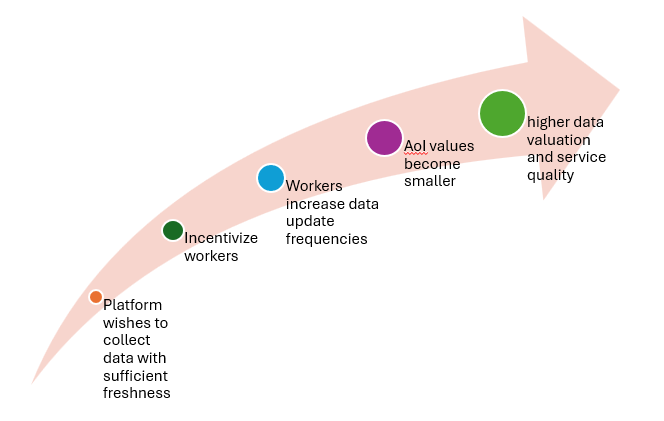
\includegraphics[width=0.5\linewidth]{incentive_flow.png} \pause
    %    \caption{Enter Caption}
    %    \label{fig:enter-label}
    \end{figure}

    \begin{itemize}
        \setlength{\itemsep} % {0.5cm} % Adjust spacing between bullets
        \item Increasing data update frequency can result in higher worker costs and congestion on the receiving data platform queues.\\ \pause
        
        \item Incomplete information – workers social relationships unknown or incomplete.\\
        
    \end{itemize}

\end{frame}

%------------------------------------------------
%\subsection{Major Contributions}
%------------------------------------------------

\begin{frame}[fragile]{Major Contributions}
    \footnotesize % Adjust font size for this frame
    \begin{itemize}[<+-| alert@+>]
        \setlength{\itemsep}{0.3cm} % Adjust spacing between bullets
        \item Solving the problem of incentive mechanism design for MCS systems with data freshness concerns using novel incomplete information two-stage Stackelberg game with constraints, while considering workers' social benefits. 
        
        \item Utilize AoI metric to measure the freshness of data and derive the closed-form expression for the AoI of the data each worker uploads to the platform taking workers’ social influences into account.
        
        \item Propose AIM, when all participants share the utility function parameters of the Stackelberg
        game. By deriving the optimal strategy for each participant, AIM can ensure that the platform and workers obtain their maximum utilities. Also theoretically prove that these optimal strategies constitute a unique Stackelberg equilibrium.
        
        \item Propose  DIM, when each participant has no prior knowledge of the game. Based on the DRL technique, DIM enables learning the optimal strategy directly from game experiences.
        
        \item Demonstrate effectiveness of the proposed AIM and DIM mechanisms' performance using real-world traces simulation.

    \end{itemize}
    %\vspace{1cm} % Add space at the bottom
\end{frame}

%------------------------------------------------
\section{System Model}
%------------------------------------------------

\begin{frame}[fragile]{System Model}
    \footnotesize % Adjust font size for this frame

    \begin{figure}
        \centering
        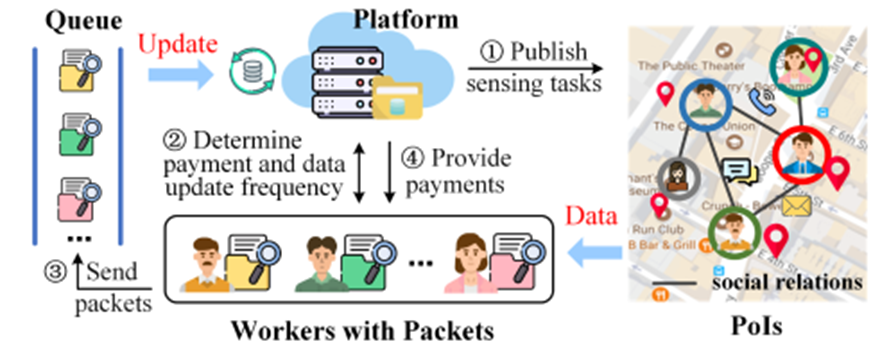
\includegraphics[width=0.6\linewidth]{system_model.png}
    %   \caption{Enter Caption}
    %   \label{fig:enter-label}
    \end{figure}\pause
    
    \begin{itemize}
        \setlength{\itemsep} % {0.5cm} % Adjust spacing between bullets
        \item Workers denoted by \( N \triangleq \{1, 2, \ldots, N\} \).\\ \pause
        \item Data Update Frequency (\(p_i\)): Rate at which worker \(i\) uploads data.\\ \pause
        \item Unit-Remuneration (\(R_i\)): Payment per update frequency to worker \(i\).    
    \end{itemize}

\end{frame}


%------------------------------------------------
%\subsection{Utility Functions}
%------------------------------------------------

% %------------------------------------------------
% \subsection{Platform Utility Functions}
%------------------------------------------------


\tikzstyle{every picture}+=[remember picture]
\everymath{\displaystyle}

\begin{frame}[fragile]{Utility Functions - Platform}
    \footnotesize % Adjust font size for this frame
    \tikzstyle{na} = [baseline=-.5ex]

    % Plain equation appears first
    \onslide<1>{
        Platform Utility Function: 
        \[
        \Phi(p_i, R_i; \eta, c, d) = \eta \sum_{i=1}^N \left(cp_i - dp_i^2\right) - \sum_{i=1}^N R_i p_i
        \]
    }

    % Highlighted equation appears in the same location
    \onslide<2->{
        \vspace{-1.5cm} % Adjust vertical space to align equations
        Platform Utility Function: 
    
        \begin{equation*}
            \Phi(p_i, R_i; \eta, c, d) = 
            \tikz[baseline]{
                \node[fill=blue!20,anchor=base] (t1)
                {$\eta$};
            } \sum_{i=1}^{N} 
            \tikz[baseline]{
                \node[fill=green!20, ellipse,anchor=base] (t2)
                {$(cp_i - dp_i^2)$};
            } - \sum_{i=1}^{N}
            \tikz[baseline]{
                \node[fill=red!20,anchor=base] (t3)
                {$R_i p_i$};
            }
        \end{equation*}
    }

    \vspace{0.5cm}

    % Incremental bullet points with synchronized arrows
    \onslide<3->{
        \begin{itemize}[<+-| alert@+>]
            \item \onslide<3->{\(\eta\): weight for platform's revenue from data 
                \tikz[na]\node [coordinate] (n1) {};} % Node appears with the bullet
            \item \onslide<4->{\((cp_i - dp_i^2)\): revenue from worker \(i\)'s data updates
                \tikz[na]\node [coordinate] (n2) {};} % Node appears with the bullet
            \item \onslide<5->{\(R_i p_i\): cost of remuneration paid to worker \(i\) 
                \tikz[na]\node [coordinate] (n3) {};} % Node appears with the bullet
        \end{itemize}
    }
    
    % Draw arrows at the same time as the corresponding bullet appears
    \begin{tikzpicture}[overlay]
        \path[->]<3-> (n1) edge [bend left] (t1);  % Arrow for the first bullet
        \path[->]<4-> (n2) edge [bend right] (t2); % Arrow for the second bullet
        \path[->]<5-> (n3) edge [out=0, in=-90] (t3); % Arrow for the third bullet
    \end{tikzpicture}
    
\end{frame}

%------------------------------------------------


% %------------------------------------------------
% \subsection{Worker Utility Functions}
%------------------------------------------------

%\tikzstyle{every picture}+=[remember picture]
%\everymath{\displaystyle}

\begin{frame}[fragile]{Utility Functions - Worker}
    \footnotesize % Adjust font size for this frame
    \tikzstyle{na} = [baseline=-.5ex]

    % Plain equation appears first
    \onslide<1>{
        Worker Utility Function: 
        \[
        \Omega_i(p_i, P_{-i}; s_i, a_i, b_i) = R(p_i) + \Psi_i(p_i, P_{-i}) - \Theta_i(p_i; s_i, a_i, b_i)
        = R_ip_i + \sum_{j \in N_i} \nu_{ij}p_ip_j - s_i(a_ip_i^2 + b_ip_i)
        \]
    }

    % Highlighted equation appears in the same location
    \onslide<2->{
        \vspace{-1.5cm} % Adjust vertical space to align equations
        Worker Utility Function: 
    
        \begin{equation*}
            \Omega_i(p_i, P_{-i}; s_i, a_i, b_i) =  
            \tikz[baseline]{
                \node[fill=blue!20,anchor=base] 
                {$R(p_i)$};
            } + 
            \tikz[baseline]{
                \node[fill=green!20, ellipse,anchor=base] 
                {$\Psi_i(p_i, P_{-i})$};
            } - 
            \tikz[baseline]{
                \node[fill=red!20,anchor=base] 
                {$\Theta_i(p_i; s_i, a_i, b_i)$};
            } =
            \tikz[baseline]{
                \node[fill=blue!20,anchor=base] 
                {$R_ip_i$};
            } + 
            \tikz[baseline]{
                \node[fill=green!20, ellipse,anchor=base] 
                {$\sum_{j \in N_i} \nu_{ij}p_ip_j$};
            } - 
            \tikz[baseline]{
                \node[fill=red!20,anchor=base] 
                {$s_i(a_ip_i^2 + b_ip_i$};
            } 
        \end{equation*}
    }

    % Incremental bullet points with synchronized arrows
    \begin{itemize}[<+->]
        \setlength{\itemsep}{0.3cm} % Adjust spacing between items
    
        % First item
        \item \onslide<3->{\(R(p) = R_ip_i\) the remuneration platform pays to worker \(i\).}
    
        % Second item
        \item \onslide<4->{\(\Psi_i(p_i, P_{-i}) = \sum_{j \in N_i} \nu_{ij} p_i p_j\) social benefits of worker \(i\).}
    
        % Third item
        \item \onslide<5->{\(\Theta_i(p_i; s_i, a_i, b_i) = s_i(a_ip_i^2 + b_ip_i)\) cost function of worker \(i\).}
    \end{itemize}
     
\end{frame}

%------------------------------------------------
\section{Problem Formulation}
%------------------------------------------------

\begin{frame}[fragile]{Two-stage Stackelberg game}
    \footnotesize % Adjust font size for this frame
    \begin{itemize}[<+-| alert@+>]
        \setlength{\itemsep}{0.5cm} % Adjust spacing between bullets
        
        \item Two-stage Stackelberg game, \(  SG\bigl(p_i, R_i; \varphi\bigr)\), where $\varphi = \{\,s_i,a_i,b_i \mid \forall i \in \mathcal{N}\}\,\cup\,\{\eta,c,d\}$ is the set of all participants' parameters, with public (SPP) and unknown parameters (SUP).\\ 

        \item Stackelberg Equilibrium (SE) with AoI Constraints: An optimal incentive strategy $\langle p_i^*, R_i^* \rangle$ constitutes a SE iff the following set of inequalities is satisfied:

            \begin{itemize}% Start of sub-bullets
                \setlength{\itemsep}{0.2cm} % Adjust spacing between bullets
                \item Leader: Platform (determines payment strategy) 
                \[
                \Phi\bigl(p_i^*, R_i^*; \eta, c, d\bigr)
                \;\ge\;
                \Phi\bigl(p_i, R_i; \eta, c, d\bigr).
                \]
                
                \item Followers: Workers (determine data update frequencies)
                \[
                \Omega_i\bigl(p_i^*, R_i^*; s_i, a_i, b_i\bigr) 
                \;\ge\;
                \Omega_i\bigl(p_i, R_i; s_i, a_i, b_i\bigr).
                \]
            
                \item Subject to: \[
                \delta_i\bigl(p_i, P_{-i}\bigr) \;\le\; \varepsilon,
                \quad \forall i \in N
                \]
                \[
                \sum_{i=1}^{n} p_i \;\le\; \hat{p}.
                \]
    
            \end{itemize}
        
    \end{itemize}
%    } % Close small font scope
\end{frame}

%------------------------------------------------
\section{Characterizing AoI of Data}
%------------------------------------------------

% %------------------------------------------------
% \subsection{AoI of Data for a Single Worker}
%------------------------------------------------

\begin{frame}[fragile]{AoI of Data for a Single Worker}
    \footnotesize % Adjust font size for this frame
    
    % Text and formula appearing first
    \onslide<1->{
        Average AoI $\overline{\delta}^T$ over the interval $[0, T]$:
        \[
        \overline{\delta}^T 
        = \frac{1}{T} \int_{0}^{T} \delta(t)\,dt 
        = \frac{1}{T}\bigl(\text{area under the AoI curve}\bigr).
        \]
    }

    % Figure appears next
    \onslide<2->{
        \begin{figure}
        \centering
        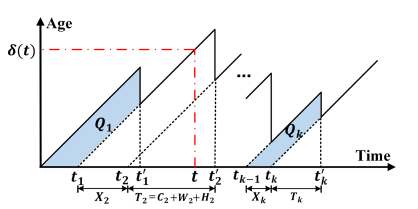
\includegraphics[width=0.5\linewidth]{AoI.png}
        \end{figure}
    }

    % Text and formula appearing after the figure
    \onslide<3->{    
        \[
        \overline{\delta}^T = \frac{1}{T} \left( Q_1 + \sum_{k=2}^{I(T)} Q_k + \frac{T_{I(T)}^2}{2} \right)
        \]

    }
\end{frame}

%------------------------------------------------
%\section{Characterizing AOI of Data}
%------------------------------------------------

% %------------------------------------------------
% \subsection{AoI of Data for a Single Worker}
%------------------------------------------------

\begin{frame}[fragile]{AoI of Data for a Single Worker (continue)}
    \footnotesize % Adjust font size for this frame
    
    \onslide<1->{    
       \hspace*{1cm} % Set a left margin of 1cm
        (12) \hspace*{2em} \(\overline{\delta}^T = \frac{1}{T} \left( Q_1 + \sum_{k=2}^{I(T)} Q_k + \frac{T_{I(T)}^2}{2} \right)
        = \frac{Q_1 + \frac{T_{I(T)}^2}{2}}{T} + \frac{I(T) - 1}{T} \cdot \frac{1}{I(T) - 1} \sum_{k=2}^{I(T)} Q_k\)
    }

    \onslide<2->{ 
    \vspace{0.3cm}
       \hspace*{1cm} % Set a left margin of 1cm
        (13) \hspace*{2em} \(Q_k = \frac{1}{2}(T_k + X_k)^2 - \frac{1}{2}T_k^2 = X_k T_k + \frac{X_k^2}{2}\)\\
    \vspace{0.5cm}
       \hspace*{1cm} % Set a left margin of 1cm
        \hspace*{4em} \(\overline{\delta}^T = \frac{Q_1 + \frac{T_{I(T)}^2}{2}}{T} + \frac{I(T) - 1}{T} \cdot \frac{1}{I(T) - 1}\sum_{k=2}^{I(T)} \left( X_k T_k + \frac{X_k^2}{2} \right)\)
    }

    \onslide<3->{ 
    \vspace{0.5cm}
       \hspace*{1cm} % Set a left margin of 1cm
        \hspace*{4em}\(p = \lim_{T \to \infty} \frac{I(T)}{T}\), indicate the data update frequency in the
steady state. \\
    \vspace{0.5cm}
        \hspace*{1cm} % Set a left margin of 1cm
        (14) \hspace*{2em}\(\overline{\delta}
        = \lim_{T \to \infty} \overline{\delta}^T
        = p\bigl(\mathbb{E}[X T] + \mathbb{E}[X^2/2]\bigr)\).
    }
   
\end{frame}

% %------------------------------------------------
% \subsection{AoI of Data for a Single Worker}
%------------------------------------------------

\begin{frame}[fragile]{AoI of Data for a Single Worker (Plugging M/M/1)}
    \footnotesize % Adjust font size for this frame
    
    For an M/M/1, FCFS queue with arrival rate $p$ and service rate $\mu$, plus an added 
    constant “collection time” $\beta$ each time a service occurs:
    \begin{itemize}
      \item Effective service-time distribution has mean \(\beta + 1/\mu\).
      \item Offered load: \(\rho = p\bigl(\beta + 1/\mu\bigr)\).
      \item Mean system time (waiting + service): \(
\mathbb{E}[T] = \frac{\beta + 1/\mu}{1 - \rho}\).
    \item Each update arrives after an exponentially distributed interarrival time \(X\), 
\(\mathbb{E}[X] = \frac{1}{p}, \quad \mathbb{E}[X^2] = \frac{2}{p^2}\)
\end{itemize}
   \hspace*{1cm} 
    \[
    \overline{\delta}
    = \frac{(\rho - 1)\bigl(\rho^2 \;-\;\mu\,\rho\,\beta\bigr) + 1}
           {\rho \,\mu \,\bigl(1 - \rho\bigr)}.
    \]
      
\end{frame}

% %------------------------------------------------
% \subsection{AoI of Data for a Multiple Workers}
%------------------------------------------------

\begin{frame}[fragile]{AoI of Data for Multiple Workers}
    \footnotesize % Adjust font size for this frame
    \tikzstyle{na} = [baseline=-.5ex]
    \onslide<1->{
        \[
        \textbf{Theorem 1: (AoI for Multiple Workers)} \\
        N \text{ workers compete for the data update through an } \text{M/M/1 FCFS queue}, \text{ in which each worker } i\text{’s data update frequency, collection time, serving rate, and offered loads are } p_i, \beta_i, \mu, \text{ and } \rho_i, \text{ respectively. Then, the average AoI } \bar{\delta}_i \text{ of worker } i\text{’s data satisfies}
        \]
    }
    \onslide<2>{
        \[
        \bar{\delta}_i = \frac{\alpha \beta_i}{\sum_{j \in \mathcal{N}_i} v_{i,j}}+ \frac{p_i}{\mu^2 (1 - \rho_{-i})} \left[ \frac{\rho_i \rho_{-i}}{(1 - \rho_{-i})^2} + \frac{\rho_i / (1 - \rho)}{1 - \rho_{-i}} + \frac{\rho_{-i}}{\rho_i} \right] + \frac{1}{\mu} + \frac{1}{p_i}
        \]
    }
    \onslide<3->{
    \vspace{-1cm}
       \begin{equation*}
            \bar{\delta}_i =   
            \tikz[baseline]{
                \node[fill=blue!20,anchor=base] (t1)
                {$\frac{\alpha \beta_i}{\sum_{j \in \mathcal{N}_i} v_{i,j}}$};
            } + 
            \tikz[baseline]{
                \node[fill=red!20, ellipse,anchor=base] (t2) 
                {$\frac{p_i}{\mu^2 (1 - \rho_{-i})} \left[ \frac{\rho_i \rho_{-i}}{(1 - \rho_{-i})^2} + \frac{\rho_i / (1 - \rho)}{1 - \rho_{-i}} + \frac{\rho_{-i}}{\rho_i} \right]$};
            } + 
            \tikz[baseline]{
                \node[fill=green!20,anchor=base]  (t3)
                {$\frac{1}{\mu} + \frac{1}{p_i}$};
            } 
        \end{equation*}
    
    }

    % Incremental bullet points with synchronized arrows
    \onslide<4->{
    \vspace{0.5cm}
        \begin{itemize}[<+-| alert@+>]
            \item \onslide<4->{\(C_k\): collection time.
                \tikz[na]\node [coordinate] (n1) {};} % Node appears with the bullet
            \item \onslide<5->{\(W_k\): wait time.
                \tikz[na]\node [coordinate] (n2) {};} % Node appears with the bullet
            \item \onslide<6->{\(H_k\): handling time. 
                \tikz[na]\node [coordinate] (n3) {};} % Node appears with the bullet
        \end{itemize}
    }
    
    % Draw arrows at the same time as the corresponding bullet appears
    \begin{tikzpicture}[overlay]
        \path[->]<4-> (n1) edge [bend left] (t1);  % Arrow for the first bullet
        \path[->]<5-> (n2) edge [bend right] (t2); % Arrow for the second bullet
        \path[->]<6-> (n3) edge [out=0, in=-90] (t3); % Arrow for the third bullet
    \end{tikzpicture}

        \vspace{-0.5cm}
       \[
        \text{where } \rho = \sum_{i=1}^N \rho_i, \quad \rho_i = \frac{p_i}{\mu}, \quad \text{and } \rho_{-i} = \sum_{j \neq i} \rho_j.
        \]
 
\end{frame}

%------------------------------------------------
\section{Bayesian Game}
%------------------------------------------------

\begin{frame}[fragile]{Bayesian Game}
    \footnotesize % Adjust font size for this frame
    \begin{itemize}[<+-| alert@+>]
        \setlength{\itemsep}{1em} % Adjust this value to control the space
        \item A \textit{Bayesian game}, or \textit{Bayesian-Nash game}, is a type of game in game theory where players have incomplete information about some aspects of the game.\\
        \item Each player is associated with a \textit{type}, which determines their preferences, payoffs, or available strategies.\\
        \item There is a commonly known prior probability distribution over the types of players.\\
        \item A strategy in a Bayesian game specifies what a player will do for every possible type they might have.\\
        \item The payoff for each player depends on their own type, their chosen action, and the types and actions of other players.\\
        \item A Bayesian Nash equilibrium is a strategy profile where each player's strategy maximizes their expected utility, given their beliefs about the other players' types and strategies.
    \end{itemize}
 
\end{frame}

%------------------------------------------------

%------------------------------------------------
 \section{AoI guaranteed Incentive Mechanism (AIM)}
%------------------------------------------------

 \begin{frame}[fragile]{AoI guaranteed Incentive Mechanism (AIM)}
     \footnotesize % Adjust font size for this frame
     Propose AoI guaranteed Incentive Mechanism (AIM) by leveraging the backward deduction approach and the KKT conditions.\\
     \vspace{0.3cm}
         \begin{enumerate}[<+-| alert@+>]
         \setlength{\itemsep}{1em} % Adjust this value to control the space
             \item Solve the worker, follower (stage-2), game.\\
             
             \begin{enumerate}
             \vspace{0.3cm}
             \setlength{\itemsep}{1em} % Adjust this value to control the space
                 \item Employ Bayesian strategy to handle incomplete information, uncertainty associated with social network effects and the strategies of other workers, by exploiting worker’s degree in the social network to derive its utility.    \\
                 
                 \item Determine worker's optimal data update frequency \(p^*_i\) under a given unit-remuneration \(R_i\).\\
                 
             \end{enumerate}
             
             \item Solve the platform, leader (stage-1) game, to derive the optimal unit-remuneration \(R^*_i\) paid by the platform.
 
         \end{enumerate}
  
\end{frame}

%------------------------------------------------
% \subsection{Solving the Bayesian Sub-Game}
%------------------------------------------------
\begin{frame}[fragile]{Solving the Bayesian Sub-Game}
     \footnotesize % Adjust font size for this frame
    \onslide<1->{    
       % \hspace*{0.5cm} % Set a left margin of 1cm
        (3) \hspace*{1em} \(\Omega_i(p_i, P_{-i}; s_i, a_i, b_i) = R(p_i) + \Psi_i(p_i, P_{-i}) - \Theta_i(p_i; s_i, a_i, b_i)
        = R_i p_i + \sum_{j \in N_i} \nu_{ij} p_i p_j - s_i \left(a_i p_i^2 + b_i p_i\right)\)
    }
    \begin{itemize}[<+-| alert@+>]
        \item Set social network influence \(\nu_{ij} = \nu\) for all \(i, j\) (\(i \neq j\)). 
        \item harness worker \(i\) degree, \(f \in G\), to describe the type of each worker. 
        \item \(\mathbb{E}[\sum_{j \in N_i} p_j] = f \times \overline{P_{-i}}\), where \(\overline{P_{-i}}\) is the average data update frequency of worker \(i\)'s neighbors.
        \item Use symmetric type space Bayesian game (i.e., workers with the same type \(f\) will choose the same data update frequency \(p(f)\) and will be awarded the same remuneration \(R(f)\).
        \item Using the "Configuration Model", randomly chosen social network neighbor of worker \(i\) has the degree distribution \(\overline{F}(f) = \frac{F(f)f}{\left(\sum_{f' \in G} F(f')f'\right)} = \frac{F(f)f}{\underline{f}}\), where \(\overline{P_{-f}} = \sum_{f \in G} \overline{F}(f)p(f).\)
        \item Thus utility of the worker with degree \(f\) can be represented as follows:
        \[
        \overline{\Omega}_f(p(f), P_{-f}) = R(f)p(f) + \upsilon p(f)f\overline{P_{-f}} - \left(a p^2(f) + b p(f)\right)s.
        \]
    \end{itemize}
  
\end{frame}

%------------------------------------------------

%------------------------------------------------
% \subsection{Follower's Optimal Strategy}
%------------------------------------------------
\begin{frame}[fragile]{Worker's (Follower) Optimal Strategy}
     \footnotesize % Adjust font size for this frame
    \onslide<1->{    
        \begin{definition}[Bayesian Nash Equilibrium (BNE)]
            A BNE is defined as a strategy profile that maximizes the expected payoff of each player for the given types and strategies performed by other players.\\ 
            A strategy vector \(\Gamma = (\Gamma_1(\psi_1), \Gamma_2(\psi_2), \dots, \Gamma_N(\psi_N))\) is a Bayesian Nash Equilibrium if and only if the following condition is satisfied for each player \(i\):
            \[
            \Gamma_i(\psi_i) \in \arg\max_{p_i \in P_i} \Omega_i(p_i, \Gamma_{-i}, \psi_i, \psi_{-i}).
            \]
        \end{definition}
    }
    \onslide<2->{    
        \begin{theorem}[Follower's Optimal Strategy]
            Given any unit remuneration \(R(f)\), the closed-form expression of the action (i.e., data update frequency) of the follower game is:
            \[
            p(f) = \frac{1}{2as} R(f) - \frac{b}{2a} + \frac{\upsilon f(\overline{R} - bs)}{2as(2as - \upsilon \overline{f})},
            \]
            where \(\overline{R} = \sum_{f \in G} \overline{F}(f)R(f)\) and \(\overline{f} = \sum_{f \in G} \overline{F}(f)f\).
        \end{theorem}
        }
\end{frame}

%------------------------------------------------
% \subsection{Platform (Leader) Game With Constraints}
%------------------------------------------------
\begin{frame}[fragile]{Platform (Leader) Game With Constraints}
    \footnotesize % Adjust font size for this frame
    \begin{itemize}[<+-| alert@+>]
        \item Platform utility function when applying the configuration model:
             \[
        \overline{\Phi} = \mathbb{E}[\Phi] = \mathbb{E} \left[ \eta \sum_{i=1}^N \left(c p_i - d p_i^2\right) - \sum_{i=1}^N R_i p_i \right] 
        = N \sum_{f \in G} F(f) \left[(\eta c - R(f)) p(f) - \eta d p^2(f)\right],
        \] 
        \item where optimizing \(\overline{\Phi}(R(f))\) with the AoI and the total update frequency constraints:\\
        \(g(R(f)) = \delta_f(R(f)) - \epsilon \leq 0,\) \hspace{0.5cm} \(g'(R(f)) = N \sum_{f} F(f)p(f) - \hat{p} \leq 0.\) \\
        
        \item Finding optimal solution, using Lagrangian function:\\
        \(\mathcal{L}(R(f), \zeta) = \overline{\Phi}(R(f)) + \zeta_1 g(R(f)) + \zeta_2 \tilde{g}'(R(f)),\) where \(\zeta_1\) and \(\zeta_2\) the Lagrangian multipliers.\\
        \vspace{0.3cm}
        \item Since it is a convex optimization problem, the optimal solution must satisfy the Karush-Kuhn-Tucker (KKT) optimality conditions:
        \[
        \frac{\partial \mathcal{L}}{\partial R(f)}\bigg|_{R(f) = R^*(f)} = 0, \quad \zeta_1 g(R(f)) = 0, \quad \zeta_2 \tilde{g}'(R(f)) = 0,
        \]
        \[
        g(R(f)) \leq 0, \quad g'(R(f)) \leq 0, \quad \zeta_1 \geq 0, \quad \zeta_2 \geq 0.
        \]
    \end{itemize} 
\end{frame}

%------------------------------------------------
% \subsection{Platform (Leader) Game With Constraints (continue)}
%------------------------------------------------
\begin{frame}[fragile]{Platform (Leader) Game With Constraints (continue)}
    \footnotesize % Adjust font size for this frame
        \onslide<1->{
            \textbf{Case 1:} $\zeta_1 = 0, \zeta_2 = 0$, both constraints are inactive.
        Plus the sum over all \( l \neq f \):
the first-order derivative of $\overline{\Phi}({R}(f))$ be equal to zero:
            \[
            \frac{\partial \overline{R}}{\partial R(f)} = \overline{F}(f), \quad 
            \frac{\partial p(l)}{\partial R(f)} = 
            \frac{\nu_l \overline{F}(f)}{2as(2as - \nu f)} = \Delta \overline{F}(f)l \quad (l \neq f),
            \]
            \[
            \frac{\partial p(f)}{\partial R(f)} = 
            \frac{1}{2as} + \frac{\nu f F(f)}{2as(2as - \nu f)} = \frac{1}{2as} + \Delta F(f)f \quad (l = f),
            \] % where \(\Delta = \frac{\nu}{2as(2as - \nu f)}\),      
        }
        \vspace{0.5cm}
        \onslide<2->{
            \[
            \frac{\partial \bar{\Phi}}{\partial R(f)} = N F(f) 
            \left[ -p(f) + (\eta c - R(f) - 2\eta dp(f)) 
            \left( \frac{1}{2as} + \Delta \overline{F}(f)f \right) \right]
            \]
            %Plus the sum over all \( l \neq f \):
            \[
            + N \sum_{l \neq f} F(l) \left[ (\eta c - R(l) - 2\eta dp(l)) \Delta \overline{F}(f)f \right] = 0.
            \]
        }
\end{frame}
%------------------------------------------------
%------------------------------------------------
% \subsection{Maximum Platform and Worker Utilities}
%------------------------------------------------
\begin{frame}[fragile]{Maximum Platform and Worker Utilities}
    \footnotesize % Adjust font size for this frame
        \onslide<1->{
            Considering social network is seen as a configuration model with large numbers of workers, optimal unit remuneration:
            \begin{align}
           & R^*(f) = \frac{2a^2 \tilde{s}^2}{
            (2as \Delta \overline{F}(f)f + 1)(as + \eta d) + as}
            \left[ \frac{b}{2a} - \Delta f (\overline{R}^* - bs) \right] 
            + \left( \Delta \overline{F}(f)f + \frac{1}{2as} \right) \nonumber \\ 
            &\left( \eta c + \frac{b\eta d}{a} - 
            2\Delta f \eta d (\overline{R}^* - bs) \right)
            + \Delta f \left[ - \left( 1 + \frac{\eta d}{as} \right) \frac{\Lambda^*}{f} 
            + \frac{\eta(ac + bd)}{a} - 2\Delta \eta d (\overline{R}^* - bs)\overline{f} \right].  \nonumber
            \end{align} 
        }
        
        \onslide<2->{
        The optimal data update frequency of worker i:
            \[
            p^*_i(f) = \frac{1}{2as} R^*(f) - \frac{b}{2a} 
            + \frac{\nu f (\overline{R}^* - bs)}{2as(2as - \nu \overline{f})}
            \]
        }
        \onslide<3->{
        \textbf{Maximum Platform and Worker Utilities}:
            \[
            \Phi^* = N \sum_{f \in G} F(f) \left[ (\eta c - R^*(f)) p^*(f) - \eta d (p^*(f))^2 \right]. 
            \]
            \[
            \Omega^*_i = R^*(f) p^*(f) + \nu p^*(f) f P_{-f} - \left( a (p^*(f))^2 + b p^*(f) \right) s.
            \]
        }
\end{frame}
%------------------------------------------------
%------------------------------------------------
% \subsection{AoL Constraint Active}
%------------------------------------------------
\begin{frame}[fragile]{AoL Constraint Active}
    \footnotesize % Adjust font size for this frame
    \onslide<1->{
            \textbf{Case 2:} $\zeta_1 \neq 0, \zeta_2 = 0$, AoI constraint \( g(R(f)) = \delta_f(R(f)) - \epsilon \leq 0 \) is active.

            \[
            g(R(f)) = \frac{\alpha \beta}{f \nu} 
            + \frac{p^2(f)}{\mu^2 \breve{\rho}} 
            \left( 
            \frac{\rho_{-i}(f)}{\mu (\breve{\rho})^2} 
            + \frac{1}{\breve{\rho} \mu (1 - \rho(f))} 
            + \frac{\rho_{-i}(f) \mu}{p^2(f)}
            \right)
            + \frac{1}{\mu} + \frac{1}{p(f)} - \epsilon = 0,
            \]
            where:
            \begin{itemize}
                \item \(\breve{\rho} = 1 - \rho_{-i}(f) \quad \text{represents the remaining service capacity.}\)
                \item \(\rho(f) = \frac{\sum_f p(f)}{\mu} \quad \text{is the total offered load.}\)
                \item \(
                 \rho_{-i}(f) = \frac{\sum_f p(f) - p(f)}{\mu} \quad \text{represents the load from other workers.}\)
            \end{itemize}
    }
    \onslide<1->{
        Since \( g(R(f)) \) depends on \( p(f) \), and \( p(f) \) is determined by \( R(f) \), combine the derivative of the utility function with the derivative of the AoI constraint to ensure both are met:
        \[
        \frac{\partial \bar{\Phi}}{\partial R(f)} + \frac{\partial g}{\partial R(f)} = 0.
        \]
    }
\end{frame}

% %------------------------------------------------
% % \subsection{AoL Constraint Active}
% %------------------------------------------------
% \begin{frame}[fragile]{AoL Constraint Active (continue)}
%     \textbf{Key Insights:}\\
    
%     \begin{itemize}
%     \setlength{\itemsep}{1em} % Adjust this value to control the space
%         \item Active constraint: The AoI constraint becomes a hard limit that the system must respect, requiring \( R(f) \) and \( p(f) \) to adjust accordingly.
%         \item Iterative solution: Since \( g(R(f)) \) is nonlinear, solving for \( R^*(f) \) typically involves numerical methods, such as Newton's method or other iterative techniques.
%         \item Impact on optimization: Enforcing \( g(R(f)) = 0 \) reduces the feasible space for optimization, potentially lowering the platform’s utility compared to the unconstrained case.\\
        
%     \end{itemize}
%     \vspace{0.3cm}
%     This case emphasizes the balance between maintaining data freshness (meeting the AoI constraint) and maximizing utility within the feasible region.
% \end{frame}

%------------------------------------------------
% \subsection{Total Data Update Frequency Constraint Active}
%------------------------------------------------
\begin{frame}[fragile]{Total Data Update Frequency Constraint Active}
    \footnotesize % Adjust font size for this frame
    \onslide<1->{
            \textbf{Case 3:} $\zeta_1 = 0, \zeta_2 \neq 0$, total data update frequency constraint \( g'(R(f)) = \sum_f F(f) p(f) - \hat{p} \leq 0 \) is active, and the system needs to adjust \( R(f) \) and \( p(f) \) to bring it back within bounds.

            \(L(R(f), \zeta_2) = \bar{\Phi}(R(f)) + \zeta_2 g'(R(f)),\) where \(g'(R(f)) = \sum_f F(f) p(f) - \hat{p}.\)
            
            For optimal \( R^*(f) \) derivative the Lagrangian with respect to \( R(f) \) and set it to zero:
            \[
            \frac{\partial \bar{\Phi}}{\partial R(f)} + \zeta_2 \frac{\partial g'}{\partial R(f)} = 0.
            \]
    }
    \onslide<2->{
        \[
        R^*(f) = \frac{as(\eta c - bs + \zeta_2)}{2as + \eta d} \left(1 - \frac{f}{\underline{f}}\right)
        + \frac{2as f \hat{p}}{N \underline{f}} + bs - 2as \Delta f (\overline{R} - bs),
        \]
        where:
        \begin{itemize}
            \item \(\bar{f} = \sum_f F(f) f \quad \text{is the average degree,}\)
            \item \(\hat{p} \quad \text{is the threshold for total update frequency,}\)
            \item \(\zeta_2 \quad \text{is determined by solving } g'(R(f)) = 0.\)
        \end{itemize}
    }
\end{frame}

%------------------------------------------------
% \subsection{Activating both constraints}
%------------------------------------------------
\begin{frame}[fragile]{Activating Both Constraints}
    \footnotesize % Adjust font size for this frame
    \onslide<1->{
        \textbf{Case 4:} $\zeta_1 \neq 0, \zeta_2 \neq 0$, AoL and total data update frequency constraints are active.
        \[
        \frac{\partial \bar{\Phi}}{\partial R(f)} 
        + \zeta_1 \frac{\partial g}{\partial R(f)} 
        + \zeta_2 \frac{\partial g'}{\partial R(f)} = 0,
        \]
        along with: \(g(R(f)) = 0, \quad g'(R(f)) = 0.\)\\
    }
    \hspace{0.5cm}
    \begin{itemize}
        \item Solving this system is complex because of nonlinearity of functions and the interdependencies betrween constraints and the utility function.\\
        
        \item Numerical methods (e.g., Bisection, Newton’s, etc.) are employed to approximate.\\
        
        \item Iterative Process.
         
    \end{itemize}
\end{frame}

%------------------------------------------------
% \subsection{The AoI-Guaranteed Incentive Mechanism (AIM)}
%------------------------------------------------
\begin{frame}[fragile]{The AoI-Guaranteed Incentive Mechanism (AIM)}
\begin{figure}
    \centering
    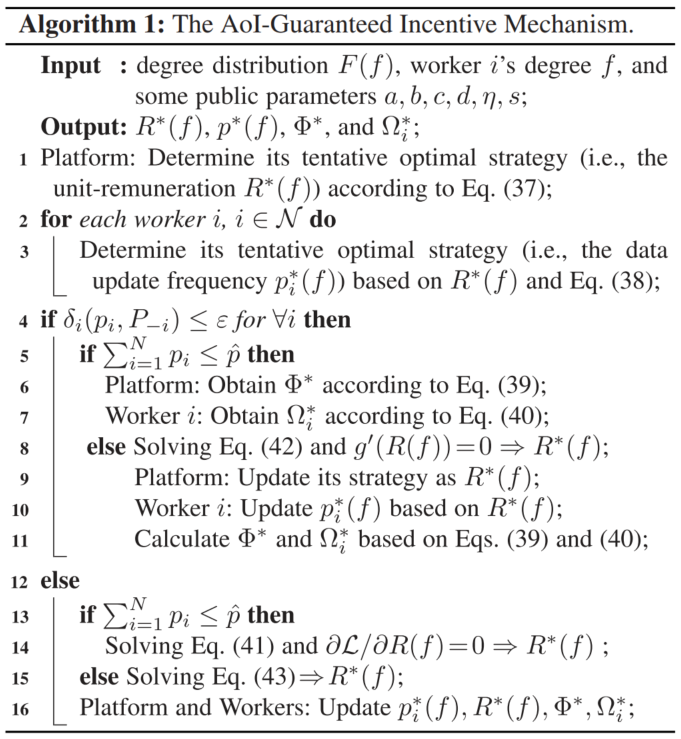
\includegraphics[width=0.4\linewidth]{AIM.png}
%    \caption{Enter Caption}
%    \label{fig:enter-label}
\end{figure}
\end{frame}

%------------------------------------------------
% \subsection{The Equilibrium Analysis}
%------------------------------------------------
\begin{frame}[fragile]{The BNE Analysis}
    \footnotesize % Adjust font size for this frame
    \textbf{Lemma 1: The follower game has at least one pure Bayesian Nash Equilibrium (BNE).}\\
    \vspace{0.3cm}
    Proof: if the Bayesian sub-game satisfies the (Milgrom-Shannon) Single Crossing Property of Incremental Returns (SCP-IR), the Bayesian subgame has at least one pure BNE.\\
    \vspace{0.3cm}
    %The SCP-IR ensures that players' payoffs increase monotonically with their own actions, given others' actions.\\
    \begin{itemize}
        \item     The partial derivative of the follower's payoff function with respect to their strategy \( p_i \) and others' strategies \( P_{-i} \) is:
            \[
            \frac{\partial^2 \bar{\Omega}_i(p_i, P_{-i}, R)}{\partial p_i \partial P_{-i}} = \nu f > 0.
            \]    
    This indicates that the payoff increases with others' strategies.\\
        \item   The second-order partial derivative with respect to \( p_i^2 \) is:
                \[
                \frac{\partial^2 \bar{\Omega}_i(p_i, P_{-i}, R)}{\partial p_i^2} = -2as < 0,
                \]
                confirming concavity of the payoff with respect to \( p_i \), which satisfies the SCP-IR. \\
    \end{itemize}    
    %\vspace{0.5cm}
\end{frame}

%------------------------------------------------
% \subsection{Stackelberg Game Equilibrium}
%------------------------------------------------
\begin{frame}[fragile]{The BNE Analysis (continue)}
    \footnotesize % Adjust font size for this frame
    \onslide<1->{
        \textbf{Lemma 2: Uniqueness of the Bayesian Nash Equilibrium}\\
        \vspace{0.3cm}
        The Bayesian sub-game has at most one BNE if the following condition is satisfied:
        \[
        \left|
        \left(
          \frac{\partial^2 \overline{\Omega}_i\bigl(p_i,P_{-i},\mathcal{R}\bigr)}
               {\partial p_i \,\partial P_{-i}}
        \right)
        \!\big/\!
        \left(
          \frac{\partial^2 \overline{\Omega}_i\bigl(p_i,P_{-i},\mathcal{R}\bigr)}
               {\partial p_i^2}
        \right)
        \right|
        < 1,
        \quad \forall\,i \in \mathcal{N}.
        \]             
        \vspace{0.3cm}
        The left-hand side represents the interaction between the strategies of player \( i \) and others.\\
        \vspace{0.3cm}
        If the interaction is sufficiently weak, the uniqueness of the equilibrium is guaranteed.\\
        \vspace{0.3cm}
        Result: When the condition \( \nu f_{\text{max}} - 2as < 0 \) is met, the uniqueness of the BNE is ensured.\\
    }
    \onslide<2->{
        \vspace{0.3cm}
        \textbf{Stackelberg Game Equilibrium:
        The leader in the Stackelberg game can optimize their strategy with the certainty that the followers' response is unique and predictable (as derived from Lemmas 1 and 2).}
    }
\end{frame}

%------------------------------------------------
% \subsection{Unique Stackelberg Equilibrium}
%------------------------------------------------
\begin{frame}[fragile]{Unique Stackelberg Equilibrium}
    \footnotesize % Adjust font size for this frame
    \onslide<1->{
        \begin{theorem}[Unique Stackelberg Equilibrium]
            The optimal incentive strategy \( \langle p^*(f), R^*(f) \rangle \) determined by AIM constitutes the unique Stackelberg equilibrium while satisfying AoI constraints.
        \end{theorem}
    }
    \onslide<1->{
    %\textbf{Proof:}\\
    \begin{itemize}
        \item \textbf{Uniqueness of Equilibrium}\\
        \begin{itemize}
            \item In Stage I, \( R^*(f) \) is derived as the unique optimal solution for the platform's utility maximization.
            \item In Stage II, \( p^*(f) \) forms a unique Bayesian Nash Equilibrium (BNE), as shown in the equilibrium analysis.
        \end{itemize}
        Together, these ensure that the entire Stackelberg game has a unique equilibrium.            
        \item \textbf{AoI Constraints} \\
              The AoI constraint, \( g(R(f)) = \delta_f(R(f)) - \epsilon \leq 0 \), ensures that the age of information for workers' data is below a specified threshold.
            This constraint is satisfied as part of the incentive mechanism design, ensuring that all workers' data meet the freshness requirement.
    \end{itemize}
    }    
\end{frame}


% %------------------------------------------------
% \section{DIM: Incentive Mechanism for SUP}
% %------------------------------------------------
% \begin{frame}[fragile]{DIM: Incentive Mechanism for SUP}
%     \footnotesize % Adjust font size for this frame
%     \begin{itemize}[<+-| alert@+>]
%         \item DRL-based Incentive Mechanism (DIM) with AoI guarantees to address the SUP problem, where the platform and workers have no prior knowledge of the Stackelberg game.
%         \item Platform conducts interactions with workers to learn the optimal strategies from game experiences.\\
%         \item Learning Framework: Twin Delayed Deep Deterministic Policy Gradient (TD3).
%         \begin{figure}
%             \centering
%             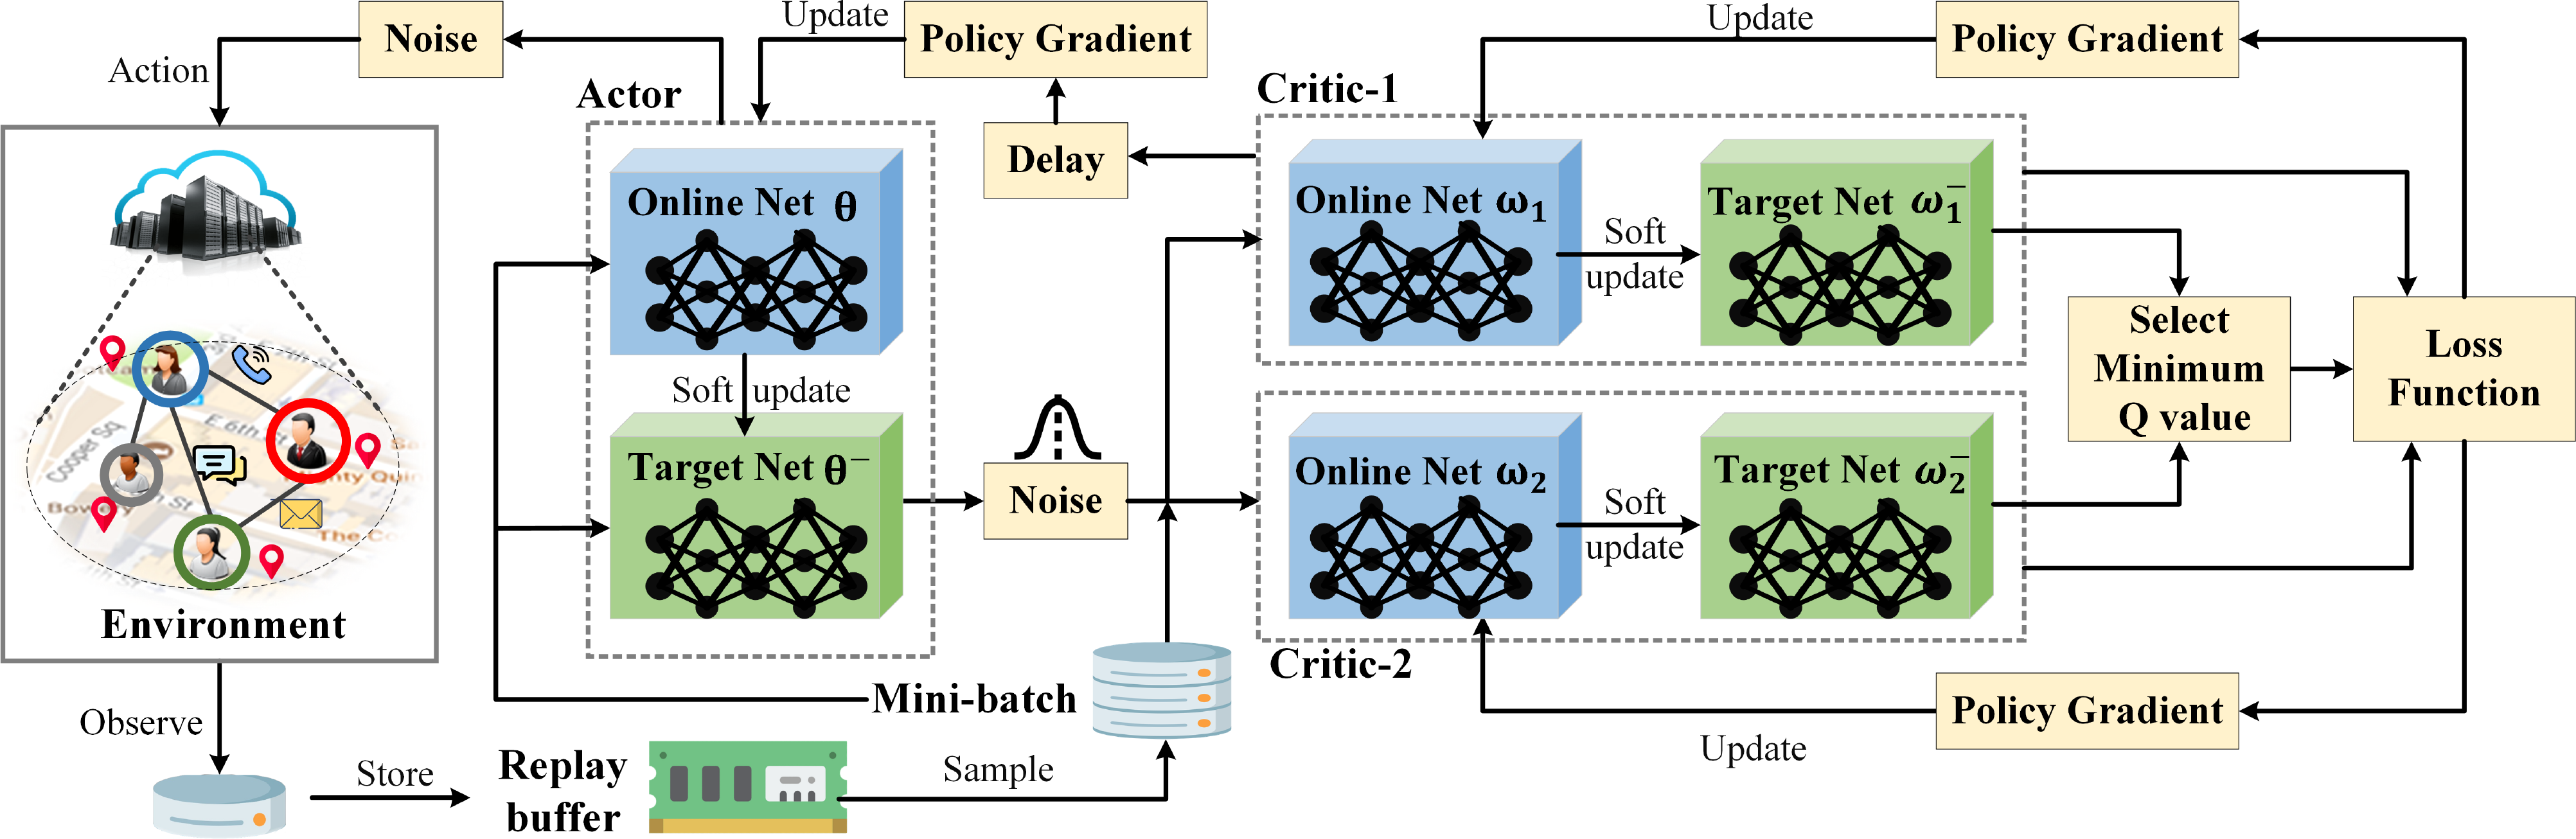
\includegraphics[width=0.7\linewidth]{DIM_learning_framework.png}
%         %   \caption{Enter Caption}
%         %   \label{fig:enter-label}
%         \end{figure}
%         \item At each time slot $t$, the platform plays the role of the game leader, announcing the payment to each worker.
%         \item Subsequently, workers act as game followers and determine their respective data update frequencies.
%     \end{itemize}     
% \end{frame}

%------------------------------------------------
\section{DRL-based Incentive Mechanism (DIM)}
%------------------------------------------------
\begin{frame}[fragile]{DRL-based Incentive Mechanism (DIM)}
    \footnotesize % Adjust font size for this frame
    \begin{itemize}[<+-| alert@+>]
        \setlength{\itemsep}{1em} % Adjust this value to control the space
        \item DRL-based Incentive Mechanism (DIM) with AoI guarantees to address the SUP problem, where the platform and workers have no prior knowledge of the Stackelberg game.
        \item Platform conducts interactions with workers to learn the optimal strategies from game experiences.\\
        \item Learning Framework: Twin Delayed Deep Deterministic Policy Gradient (TD3).
        \vspace{0.3}
        \begin{itemize}
        \footnotesize
            \setlength{\itemsep}{0.5em} % Adjust this value to control the space
            \item TD3 contains two types of networks, actor network and two critic networks.
            \item Actor network learns the policy $\pi_{\theta}(a \mid s)$, and decides what action to take in a given state.
            \item Critic network evaluates the quality, $Q(s, a)$, of the action and guide actor to improve decisions.
            \item Each actor (or critic) network is composed of two sub-networks: online network and target network. 
            \item The target networks used to compute the target actions and the target $Q$-values of the next state. 
        \end{itemize}
    \end{itemize}     
\end{frame}

%------------------------------------------------
%\subsection{DIM Learning Framework (continue 1)}
%------------------------------------------------
\begin{frame}[fragile]{DIM Learning Framework (continue 1)}
    \footnotesize % Adjust font size for this frame
    \onslide<1->{
        \begin{figure}
            \centering
            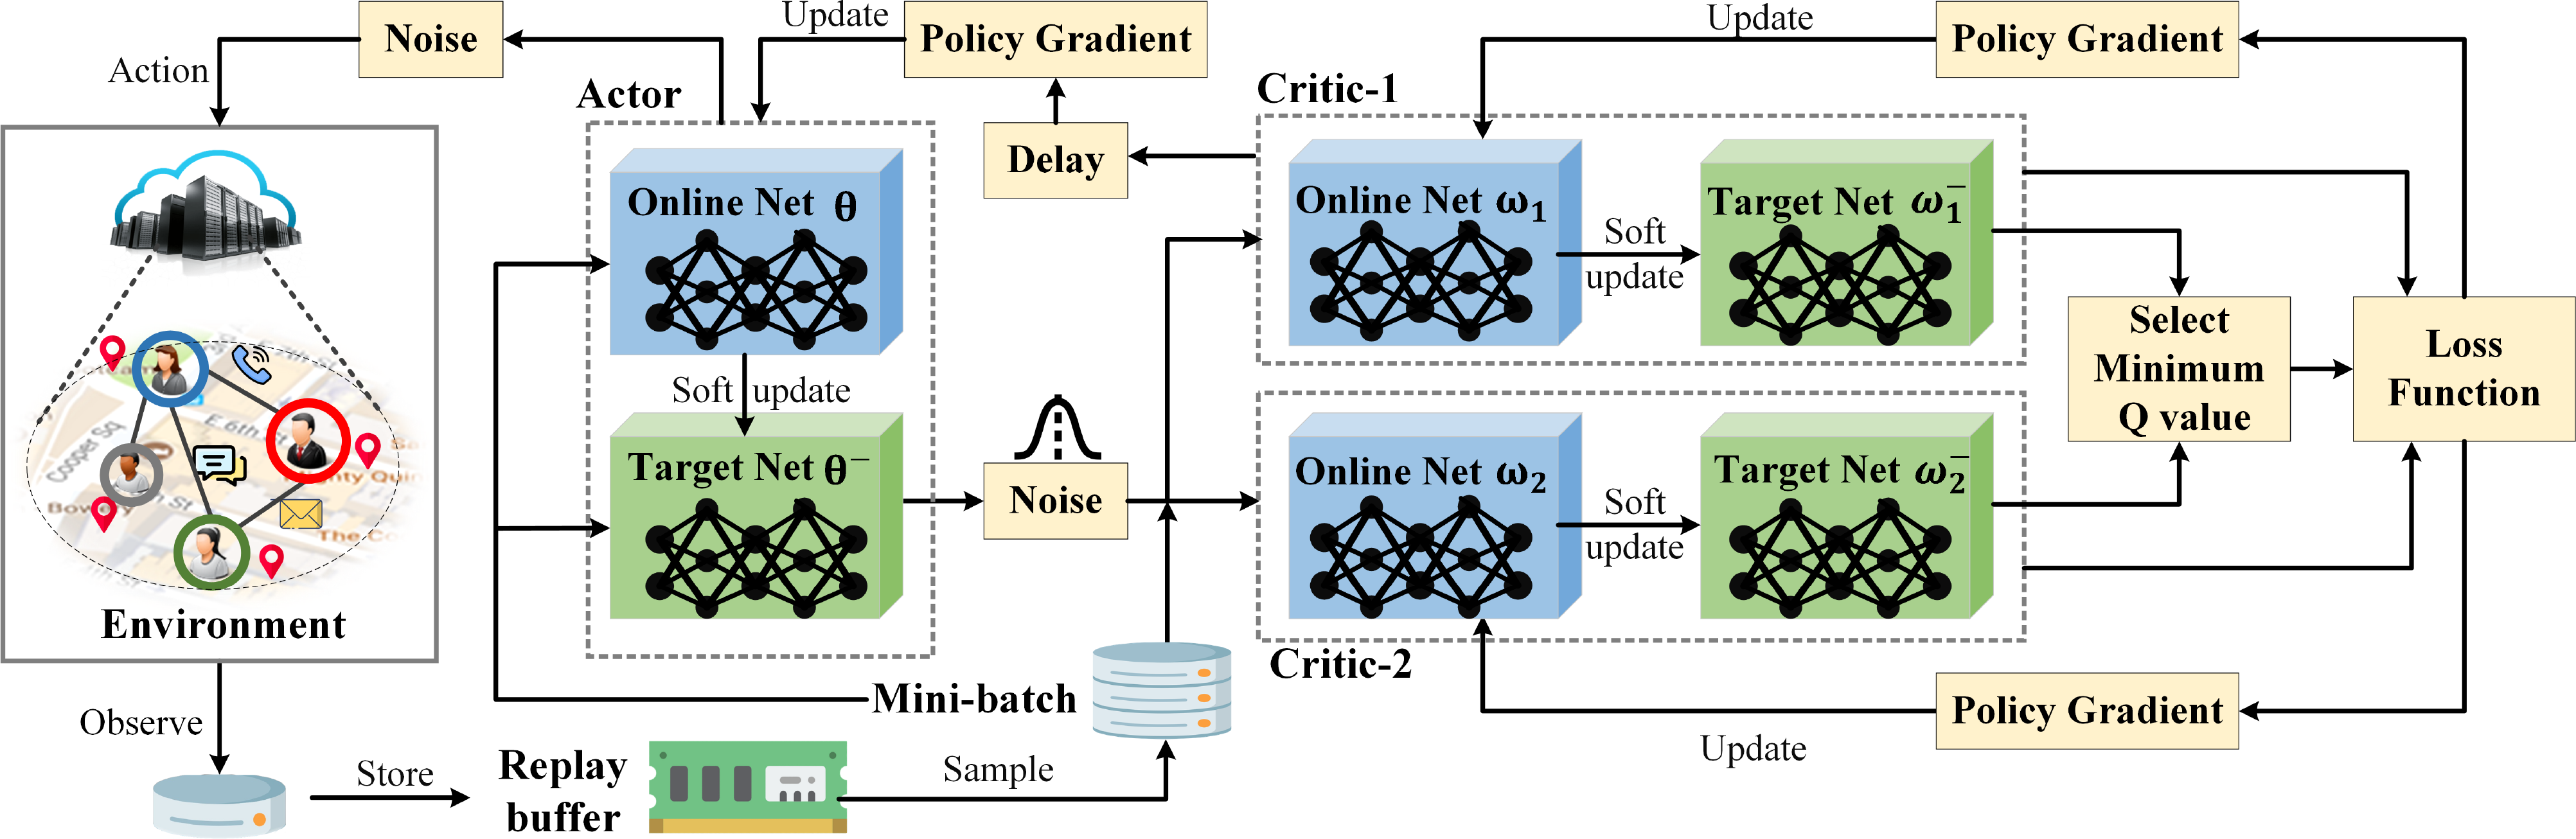
\includegraphics[width=0.8\linewidth]{DIM_learning_framework.png}
            % \caption{Enter Caption}
            % \label{fig:enter-label}
        \end{figure}
    }
    \begin{itemize}
        \onslide<2->{\item By selecting the minimum $Q$-value of the two critics target networks, TD3 can achieve more accurate value and the overestimation bias is significantly reduced.}
        \onslide<3->{\item Actor network update frequency is less than the critic networks to mitigate policy oscillations, reduce overfitting risks, and stabilize the training process.}
        \onslide<4->{\item Random noise promotes more diverse exploration and reduces the tendency to exploit a single action.}
    \end{itemize}
\end{frame}

%------------------------------------------------
%\subsection{DIM Learning Framework (continue 2)}
%------------------------------------------------
\begin{frame}[fragile]{DIM Learning Framework (continue 2)}
    \footnotesize % Adjust font size for this frame
    \begin{itemize}[<+-| alert@+>]
    \setlength{\itemsep}{1em} % Adjust this value to control the space
        \item At each time slot $t$, the platform plays the role of the game leader, announcing the
        payment to each worker.\\ Subsequently, workers act as game followers and determine their respective data update frequencies.
        \item based on the current state observed from the environment, the platform or each worker can map the state to an appropriate action and will execute the action. Upon observing the impact of the action on the environment, the platform or each worker will receive an immediate reward, and the current state is transited to the next state.
        \item The experience (i.e., current state, action, reward, and next state) is saved in the finite-size replay buffer, which used for the network update.
    \end{itemize}
\end{frame}

%------------------------------------------------
%\subsection{Payment Strategy for the Platform}
%------------------------------------------------
\begin{frame}[fragile]{Payment Strategy for the Platform}
    \footnotesize % Adjust font size for this frame
      \begin{itemize}
          \setlength{\itemsep}{1em} % Adjust this value to control the space
          \onslide<1->{\item Payment decision in the two-stage Stackelberg game is modeled as a Markov Decision Process (MDP).}
          \onslide<2->{\item MDP Freamwork:}
          \begin{itemize}
           \setlength{\itemsep}{1em} % Adjust this value to control the space
            \onslide<3->{\item State Space: includes vectors of historical payment strategies and corresponding data update frequencies over a defined number of past \(\tau\) time slots: \[
            s^t = \{R^{t-\tau}, P^{t-\tau}, R^{t-\tau+1}, P^{t-\tau+1}, \dots, R^{t-1}, P^{t-1}\}.
            \]}
            \onslide<4->{\item Action Space: platform's payment strategy at the current time slot \(t\) according to the actor network with random noise: \(R^t = \Pi_\theta(s^t) + \xi\).}
            \onslide<5->{\item Reward Function: 
                \[
                \Upsilon(\mathbf{s}^t, \mathcal{R}^t) = \varrho_1 \Phi(P^t, \mathcal{R}^t) 
                - \varrho_2 \left[\frac{\sum_{i=1}^N p_i^t - \hat{p}}{\hat{p}}\right]^+ 
                - \varrho_3 \sum_{i=1}^N \left[\frac{\delta_i^t - \epsilon}{\epsilon}\right]^+,
                \]}
          \end{itemize} 
      \end{itemize}  
\end{frame}


%------------------------------------------------
%\subsection{Payment Strategy for the Platform}
%------------------------------------------------
\begin{frame}[fragile]{Network Training}
    \footnotesize % Adjust font size for this frame
    \begin{enumerate}[<+-| alert@+>]

        \setlength{\itemsep}{1em} % Adjust this value to control the space
        
        \item Platform: picks action \( R_t \rightarrow \text{Environment (workers in parallel)} \).
        
        \item Environment: aggregates the workers’ responses  
        \(
        \rightarrow \text{ returns } (s_{t+1}, \text{reward}).
        \)

        \item Platform: stores \( \langle s_t, R_t, \text{reward}, s_{t+1} \rangle \) in replay buffer.
        
        \item Platform: (possibly) samples mini-batches from replay buffer  
        \(
        \rightarrow \text{ updates neural networks.}
        \)

    \end{enumerate}
\end{frame}

% %------------------------------------------------
% %\subsection{Payment Strategy for the Platform}
% %------------------------------------------------
% \begin{frame}[fragile]{Data Collection and Experience Replay}
%     \footnotesize % Adjust font size for this frame
% \textbf{Observe State $s_{t}$:}
% \begin{itemize}
%   \item At the start of each time slot $t$, the platform observes the current system state $s_{t}$.
% \end{itemize}

% \textbf{Select Action $R_{t}$:}
% \begin{itemize}
%   \item The actor network outputs a base action $\Pi_{\theta}(s_{t})$.
%   \item A noise term (drawn from a normal distribution) is added for exploration:
%   \[
%     R_{t} \;=\; \Pi_{\theta}(s_{t}) \;+\; \text{(Gaussian noise)}.
%   \]
% \end{itemize}

% \textbf{Execute Action \& Observe Reward $\Upsilon(s_{t},R_{t})$:}
% \begin{itemize}
%   \item After $R_{t}$ is chosen and executed, the environment returns a reward $\Upsilon(s_{t}, R_{t})$.
%   \item The system transitions to the next state $s_{t+1}$.
% \end{itemize}

% \textbf{Store Transition in Replay Buffer:}
% \begin{itemize}
%   \item The 4-tuple $\langle s_{t}, R_{t}, \Upsilon(s_{t},R_{t}), s_{t+1}\rangle$ is stored in the replay buffer.
%   \item If the buffer is full, the oldest entries are removed.
%   \item Random or prioritized sampling from this buffer helps break the correlation among consecutive experiences.
% \end{itemize}
% \end{frame}


%------------------------------------------------
\section{Performance Evaluation}
%------------------------------------------------
\begin{frame}[fragile]{Evaluation of AoI}
    \footnotesize % Adjust font size for this frame

    \begin{figure}
        \centering
        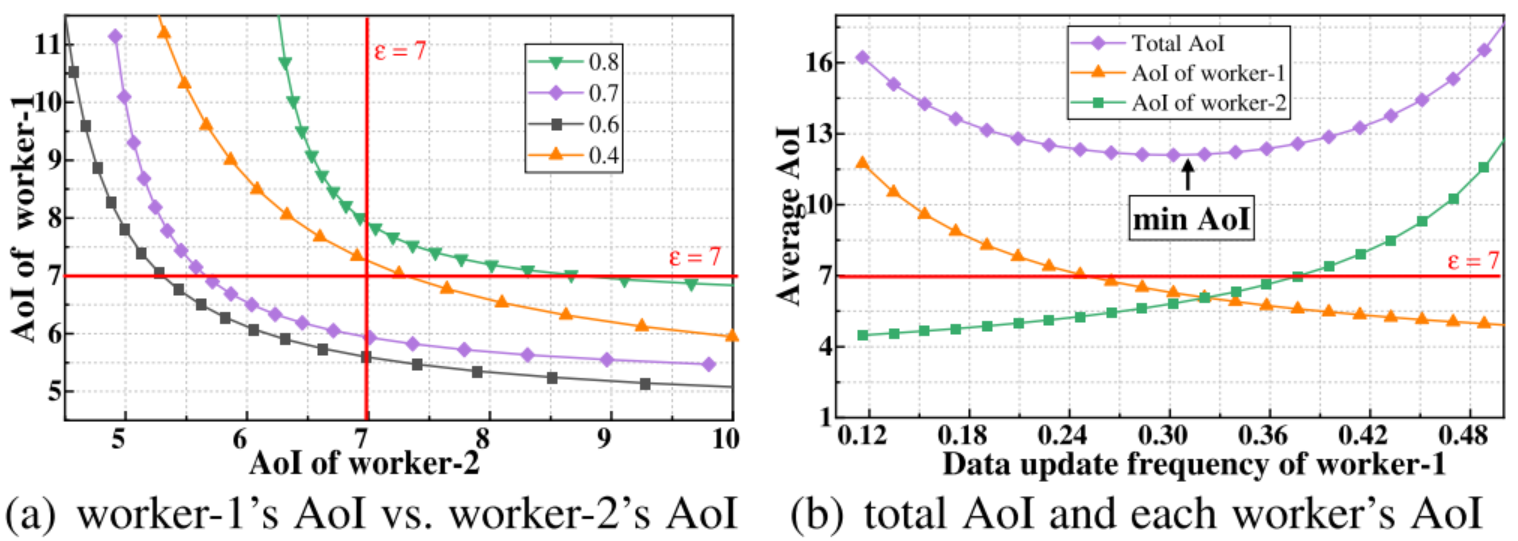
\includegraphics[width=0.8\linewidth]{Two_Worker_AoI.png}
    %   \caption{Enter Caption}
    %   \label{fig:enter-label}
    \end{figure}

    \textbf{Evaluating AoI}: two workers, fixed total load \(\rho_1 + \rho_2 = \hat{\rho}\).
    
    \begin{enumerate}[(a)]
        \item AoI value of worker-1 decreases with the increase of worker-2’s AoI value.
        %\item If we set the threshold as \(\varepsilon = 7\), workers can meet the AoI constraint only when \(\hat{\rho} = 0.6\) or \(0.7\).
        \item AoI optimization problem depends on both the total load \(\hat{\rho}\) and the allocation of data update frequency among workers.
    \end{enumerate}
\end{frame}

%------------------------------------------------
%\subsection{Evaluation of AIM}
%------------------------------------------------
\begin{frame}[fragile]{Evaluation of AIM - Platform}
    \footnotesize % Adjust font size for this frame

    \begin{figure}
        \centering
        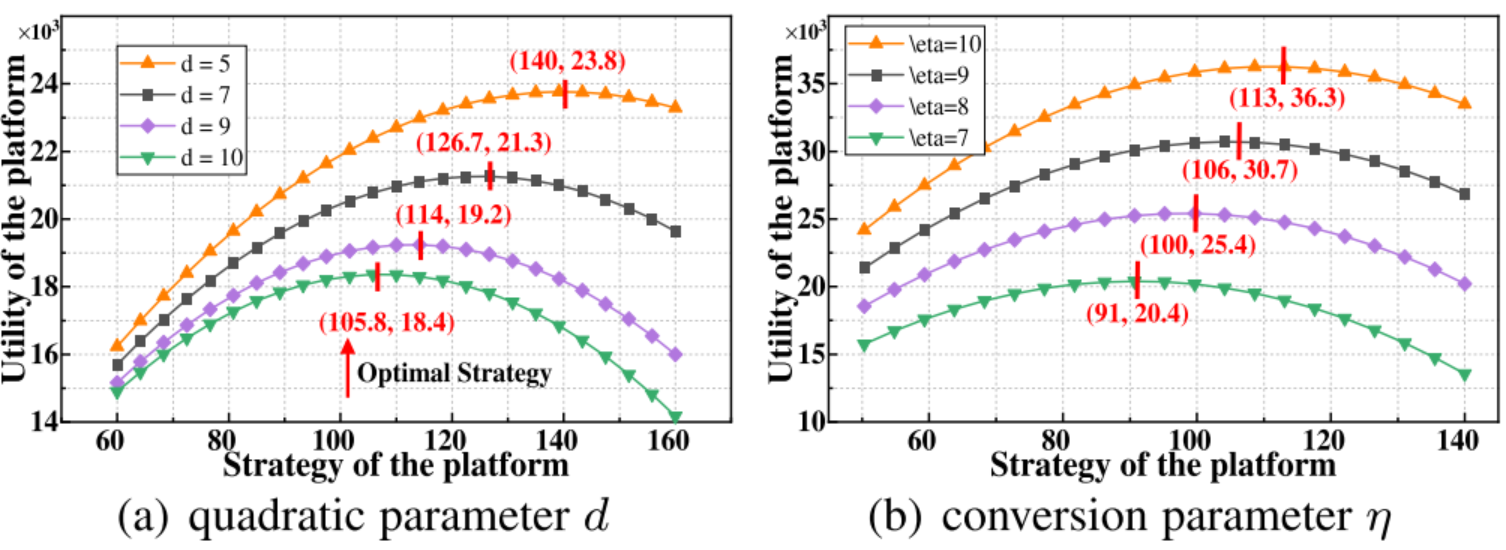
\includegraphics[width=0.8\linewidth]{performence_of_AIM.png}
    %   \caption{Enter Caption}
    %   \label{fig:enter-label}
    \end{figure}
    
    \textbf{Evaluating AIM}: Platform Strategy Vs. Utility with different parameters.
    
    \begin{itemize}
        \item PU will always find a maximum point.
        \item A small \(d\) or a larger \(\eta\) will result in the growth of the optimal \(PS\) and the optimal \(PU\).
    \end{itemize}
\end{frame}

%------------------------------------------------
%\subsection{Evaluation of AIM}
%------------------------------------------------
\begin{frame}[fragile]{Evaluation of AIM - Worker}
    \footnotesize % Adjust font size for this frame

    \begin{figure}
        \centering
        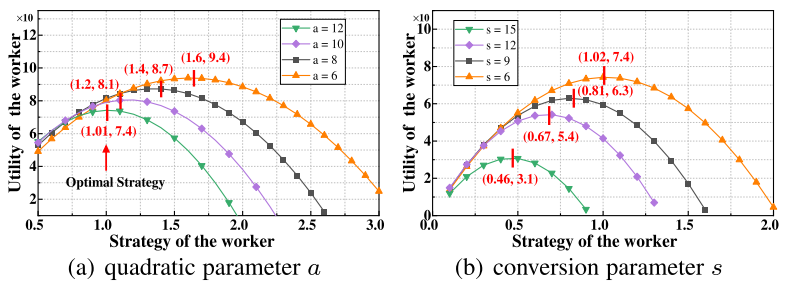
\includegraphics[width=0.8\linewidth]{Evaluation_AIM_Worker.png}
    %   \caption{Enter Caption}
    %   \label{fig:enter-label}
    \end{figure}
    
    \textbf{Evaluating AIM}: Worker Strategy Vs. Utility with different parameters.
    
    \begin{itemize}
        \item WU find a maximum point.
        \item worker’s utility increase when applying a smaller $a$ or $s$ since the cost of the
        worker becomes smaller.
    \end{itemize}
\end{frame}

%------------------------------------------------
%\subsection{Evaluation of Social Network Effect}
%------------------------------------------------
\begin{frame}[fragile]{Evaluation of Social Network Effect}
    \footnotesize % Adjust font size for this frame
    \begin{figure}
        \centering
        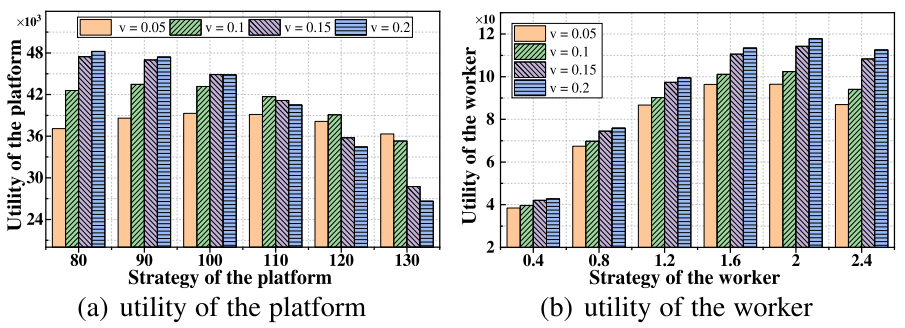
\includegraphics[width=0.8\linewidth]{Social Network Effects.png}
    %    \caption{Enter Caption}
    %    \label{fig:enter-label}
    \end{figure}    
    \textbf{Evaluating Influence of social network effects}: 
    
    \begin{itemize}
        \item Enlarging social network effect coefficient \(\upsilon\) from 0.05 to 0.2, enables both the worker and platform to achieve higher utility.
    \end{itemize}
\end{frame}

%------------------------------------------------
%\subsection{Evaluation of Different Incentive Mechanisms}
%------------------------------------------------
\begin{frame}[fragile]{Evaluation of Different Incentive Mechanisms}
    \footnotesize % Adjust font size for this frame
    \textbf{Evaluation of Different Incentive Mechanisms}: 
\begin{figure}
        \centering
        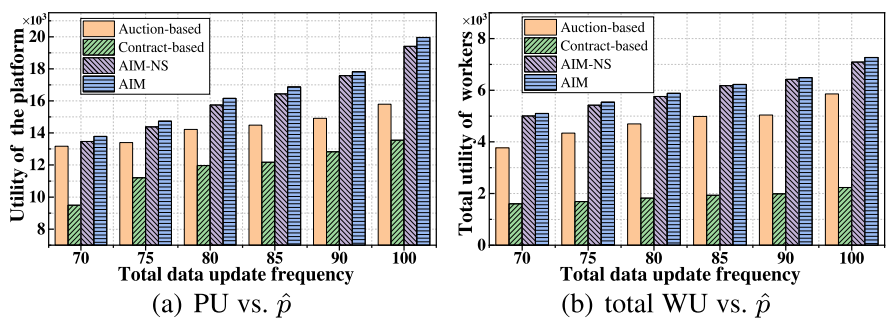
\includegraphics[width=0.8\linewidth]{different_incentive_mechanisms.png}
    %   \caption{Enter Caption}
    %   \label{fig:enter-label}
    \end{figure}
        
    \begin{itemize}
        \item When $\hat{p} = 100$, the achieved PU of AIM is about 47.3\% and 26.4\% higher than those of the contract-based and auction-based algorithms on average, respectively.
    \end{itemize}
\end{frame}

%------------------------------------------------
%\subsection{Evaluation of DIM Conversion}
%------------------------------------------------
\begin{frame}[fragile]{Evaluation of DIM Conversion}
    \footnotesize % Adjust font size for this frame
    \textbf{Evaluation of DIM Conversion via training loss}: 
\begin{figure}
            \centering
            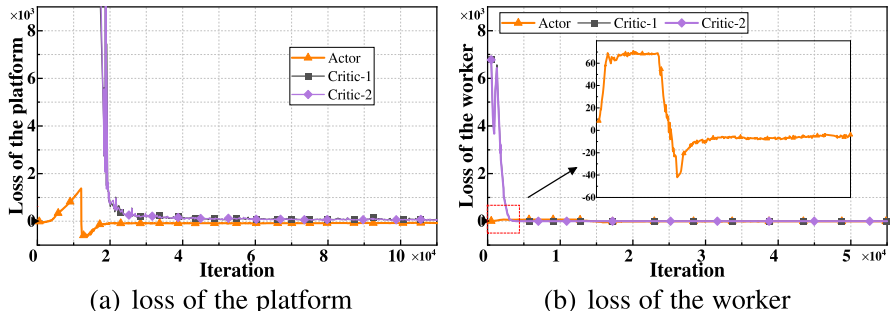
\includegraphics[width=0.8\linewidth]{DIM_conversion.png}
        %   \caption{Enter Caption}
        %   \label{fig:enter-label}
        \end{figure}        
    \begin{itemize}
        \item Both the actor network and two critic networks of the platform tend to a stable state as the training time increases.
    \end{itemize}
\end{frame}


%------------------------------------------------
\section{Conclusion}
%------------------------------------------------
\begin{frame}[fragile]{Conclusion}
    \footnotesize % Adjust font size for this frame
    \onslide<1->{\textbf{Modeling Approach:}
    The problem is framed as a two-stage Stackelberg game with an embedded Bayesian sub-game to account for incomplete information.}\\
    \vspace{0.3cm}
    \onslide<2->{\textbf{Proposed Mechanisms:}}
   
    \begin{itemize}
        \onslide<3->{\item \textbf{AIM (AoI-guaranteed Incentive Mechanism):}}
        \begin{itemize}
            \onslide<4->{\item Designed for scenarios where participants share utility function parameters.
            \item Ensures unique Stackelberg equilibrium and maximizes the utilities of both the platform and workers.}
        \end{itemize}
        \onslide<5->{\item \textbf{DIM (DRL-based Incentive Mechanism):}}
        \begin{itemize}
            \onslide<6->{\item Extended for scenarios with no prior knowledge of utility parameters.
            \item Utilizes Deep Reinforcement Learning (DRL) to enable participants to learn optimal strategies through experience.
            \item Ensures AoI values remain within a specified threshold.}
        \end{itemize}
    \end{itemize}
    
    \vspace{0.3cm}
    \onslide<7->{\textbf{Performance Evaluation:}}  
    \begin{itemize}
        \onslide<8->{\item Experiments with real-world data validate the efficacy of AIM and DIM.
        \item Both mechanisms outperform baseline methods in utility optimization and AoI guarantee.}
    \end{itemize}
      \vspace{0.3cm}  
\end{frame}


%------------------------------------------------
\section{My Contribution}
%------------------------------------------------
 \begin{frame}[fragile]{My Contribution}
    \footnotesize % Adjust font size for this frame
    \onslide<1->{\textbf{Areas for improvements:}}\\
    \begin{itemize}
        \onslide<2->{\item Practical Applicability: The paper focuses on theoretical formulations and simulations but does not sufficiently address the challenges of implementing AIM or DIM in real-world MCS systems.}
        \onslide<3->{\item Social Benefit Modeling: The paper assumes stable social relationships and fixed system parameters, which may not reflect the dynamic nature of real-world systems.}\\ 
    \end{itemize}

    \vspace{0.3cm}
    \onslide<4->{\textbf{Future Directions:}}
    \begin{itemize}
        \onslide<5->{\item Explore social interaction models, such as time-varying influence networks or dynamic feedback from workers.}\\
        \onslide<6->{\item Propose mechanisms to integrate other metrics beyond AoI (e.g., data quality or energy efficiency).}
        \onslide<7->{\item Investigate the impact of collaborative behavior among workers.}
    \end{itemize}
\end{frame}

%=======================================================================================
\end{document}